\documentclass[a4paper]{oblivoir}
\usepackage{amsmath,amssymb,kotex,kswrapfig,mdframed,paralist}
\usepackage{fapapersize}
\usefapapersize{210mm,297mm,20mm,*,20mm,*}

\usepackage{tabto,pifont}
\TabPositions{0.2\textwidth,0.4\textwidth,0.6\textwidth,0.8\textwidth}
\newcommand\tabb[5]{\par\noindent
\ding{172}\:{\ensuremath{#1}}
\tab\ding{173}\:\:{\ensuremath{#2}}
\tab\ding{174}\:\:{\ensuremath{#3}}
\tab\ding{175}\:\:{\ensuremath{#4}}
\tab\ding{176}\:\:{\ensuremath{#5}}}

\usepackage{graphicx}

\pagestyle{empty}

%%% Counters
\newcounter{num}

%%% Commands
\newcommand\prob[1]
{\bigskip\par\noindent\stepcounter{num} \textbf{문제 \thenum) #1}\par\noindent}

\newcommand\pb[1]{\ensuremath{\fbox{\phantom{#1}}}}

\newcommand\ba{\ensuremath{\:|\:}}

\newcommand\vs[1]{\vspace{25pt}}

\newcommand\an[1]{\bigskip\par\noindent\textbf{문제 #1)}\par\noindent}

%%% Meta Commands
\let\oldsection\section
\renewcommand\section{\clearpage\oldsection}

\let\emph\textsf

\begin{document}
\begin{center}
\LARGE준영, 미니테스트 11
\end{center}
\begin{flushright}
날짜 : 2017년 \(\pb3\)월 \(\pb{10}\)일 \(\pb{월}\)요일
,\qquad
제한시간 : \pb{17년}분
,\qquad
점수 : \pb{20} / \pb{20}
\end{flushright}

%
\prob{}
다음 중 그 값이 가장 큰 것은?
(단, \([x]\)는 \(x\)보다 크지 않은 최대의 정수이다.)
\tabb%
{\displaystyle\lim_{x\to0-}\frac{[x-2]}{x-2}}
{\displaystyle\lim_{x\to0+}\frac{x}{[x-1]}}
{\displaystyle\lim_{x\to-1+}\frac{[x]^2-1}{[x^2-1]}}
{\displaystyle\lim_{x\to1-}\frac{[x-2]}{[x+1]}}
{\displaystyle\lim_{x\to\infty}\left[\frac{2x+1}{x+1}\right]}
\vs

%
\prob{}
\(x\)에 대한 다항식 \(f(x)\)가
\[\lim_{x\to\infty}\frac{f(x)-4x^2}{2x-3}=a,\qquad
\lim_{x\to1}\frac{f(x)}{x-1}=-2\]
를 만족시킬 때, 상수 \(a\)의 값은? (단 \(a\neq0\))
\vspace{10pt}
\tabb{-10}{-8}{-5}{-3}{-2}
\vs

%
\prob{}
아래 그림과 같이 함수 \(y=2x^2\)의 그래프 위의 점 \(P(t,2t^2)\)에 대하여 점 \(P\)를 지나고 직선 \(OP\)와 수직인 직선이 \(y\)축과 만나는 점의 \(y\)좌표를 \(f(t)\)라 할 때, \(\displaystyle\lim_{t\to0}f(t)\)의 값을 구하여라.
(단, \(O\)는 원점이다.)

\begin{figure*}[h!]
\centering
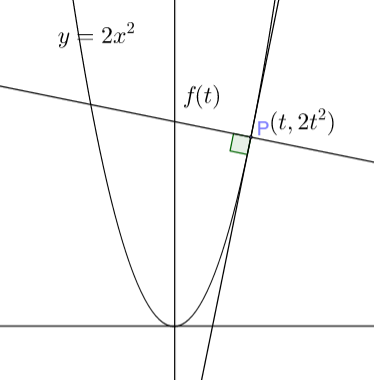
\includegraphics[width=0.3\textwidth]{123}
\end{figure*}

\end{document}